\documentclass{article}
\usepackage{geometry}
\geometry{a4paper, margin=1in}
\usepackage{graphicx}
\usepackage{hyperref}

% Create title page
\title{\vspace*{100pt}CSCI4100U: Mobile Devices \\ \underline{Project Proposal} \vspace*{30pt}}
\author{
    Syed Naqvi \\ 
    Brendan Murray \\ 
    Evan Goldberg
    \vspace*{30pt}
}
\date{\today}

\begin{document}

% Title page
\maketitle
\newpage

% Table of contents
\tableofcontents
\newpage

\section{Overview}
The purpose of this document is to propose the development of a mobile application titled \textbf{Task Bell}.
This app offers an effective and local solution for shift-workers as well as individuals requiring multitasking
or productivity management assistance.

\section{Core Features}
This section outlines the key features and functionalities of the proposed mobile application.
\begin{itemize}
    
    \item \textbf{Alarm Grouping:}\\The ability to create a hierarchical alarm grouping structure, similar to a directory tree,
    that can be used to set multiple alarms at once. Settings of a parent group can be applied locally or propagated to all child groups.
    Individual groups or alarms can optionally be set to 'inheritance blocking mode' making them immune from any propagated settings.

    \item \textbf{Date/Time - Based Recurrence Settings:}\\The user will be able to set recurrence patterns for their alarms/groups based on
    calendar dates and times of the day.

    \item \textbf{Location - Based Recurrence Settings:}\\The user can choose to make their alarms/groups recur based on their location.
    
    \item \textbf{Alarm Disabling Tasks:}\\The alarms/groups can be set so that tasks such as object/QR code scanning or puzzle completion
    are required before any particular alarm can be disabled.

    \item \textbf{Timer/Stopwatch Support:}\\The app will allow standard stopwatch and timer support including multiple stopwatches and/or
    timers running simultaneously.

\end{itemize}

\section{Technical Specifications}
The app will be built using the following technologies:
\begin{itemize}
    \item \textbf{Programming Languages:} Dart
    \item \textbf{Frameworks:} Flutter
    \item \textbf{Platforms:} Android platform
    \item \textbf{Database:} SQLite
    \item \textbf{APIs:} Fused Location Provider API, Google Maps Android API, Geofencing API, Dart:Core - DateTime API
\end{itemize}

\section{Work Distribution}
The planned workload distribution is as follows:\\

\begin{tabular}{|p{3cm}|p{4cm}|p{7cm}|}
    \hline
    \textbf{Team Member} & \textbf{Task} & \textbf{Description} \\
    \hline
    Syed Naqvi      & [Task] & [Description] \\
    Evan Goldberg   & [Task] & [Description] \\
    Brendan Murray  & [Task] & [Description] \\
    \hline
\end{tabular}

\newpage

\section{UML Diagrams}
The following UML diagrams are intended to provide an overview of the application design:
% Add an image
\begin{figure}[h!]
    \centering
    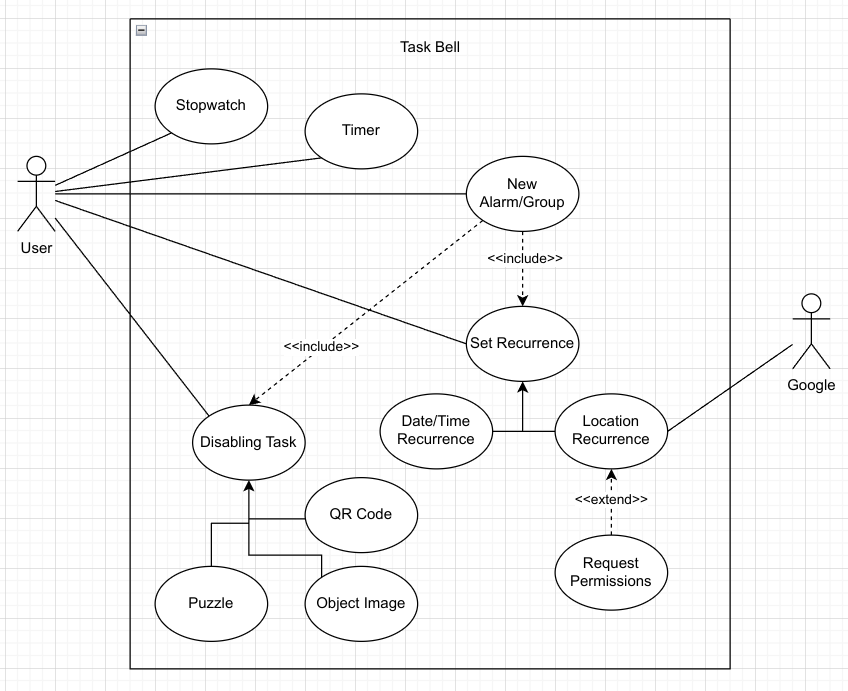
\includegraphics[width=0.6\textwidth, height=0.3\textheight]{../Use_Case_Diagram.png}
    \caption{Use Case Diagram}
    \label{fig:example_image}
\end{figure}
\begin{figure}[h!]
    \centering
    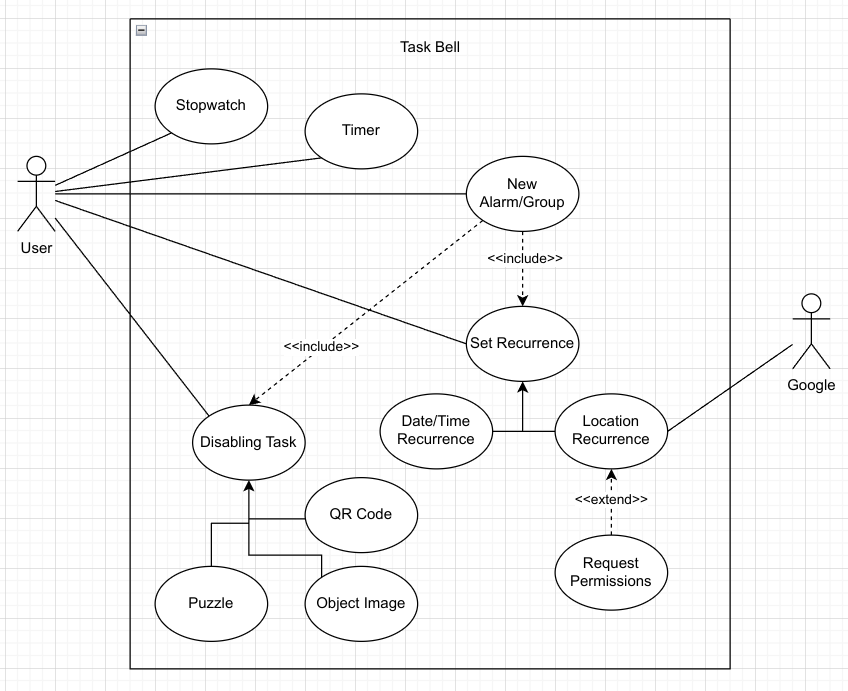
\includegraphics[width=0.6\textwidth, height=0.3\textheight]{../Use_Case_Diagram.png}
    \caption{Design Class Diagram}
    \label{fig:example_image}
\end{figure}

\section{Mockup User Interface}
This is a rough overview of the proposed user-interface:


\end{document}
